\begin{figure}[H]
  \centering

  \begin{subfigure}[b]{0.2\textwidth}
    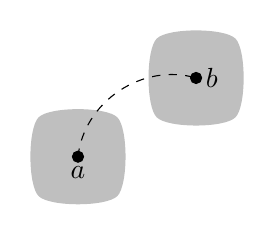
\begin{tikzpicture}
      \fill [lightgray] plot [smooth cycle] coordinates {
        (0, 0) (0, 1)  (1, 1) (1, 0)
      };
      \fill [lightgray] plot [smooth cycle] coordinates {
        (2.5, 1) (2.5, 2)  (1.5, 2) (1.5, 1)
      };
      \draw[dashed] (0.5, 0.5) edge[bend left = 50] (2, 1.5);
      \draw[fill = black] (0.5, 0.5) circle (2pt) node[below] {\(a\)};
      \draw[fill = black] (2, 1.5) circle (2pt) node[right] {\(b\)};
    \end{tikzpicture}

  \caption{Несвязная область}\label{fig:area-prop-3-a}
  \end{subfigure}
  \qquad
  \begin{subfigure}[b]{0.2\textwidth}
    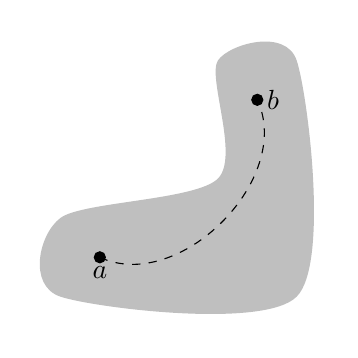
\begin{tikzpicture}

      \fill [lightgray] plot [smooth cycle] coordinates {
        (0, 0) (0, 1) (2, 1.5) (2, 3) (3, 3) (3, 0)
      };
      \draw[dashed] (0.5, 0.5) edge[bend right = 70] (2.5, 2.5);
      \draw[fill = black] (0.5, 0.5) circle (2pt) node[below] {\(a\)};
      \draw[fill = black] (2.5, 2.5) circle (2pt) node[right] {\(b\)};

    \end{tikzpicture}
    \caption{Связная область}\label{fig:area-prop-3-b}
  \end{subfigure}
\end{figure}
